%example

\begin{frame}
  \frametitle{鲸鱼优化算法}

	 \begin{enumerate}
	    \item 面向问题
	    \item 灵感来源
	    \item 模型建立
	    \item 算法步骤
	    \item 评价
	  \end{enumerate}
\begin{picture}(1,1)
\put(75,0){
\includegraphics[width=0.6\textwidth]{pic/whale_author.png}}
\end{picture}
\end{frame}


\begin{frame}
  \frametitle{要解决什么优化问题?}
	\begin{itemize}
	\item {形如各种基准函数的优化问题}
	\end{itemize}
\begin{figure}
\centering
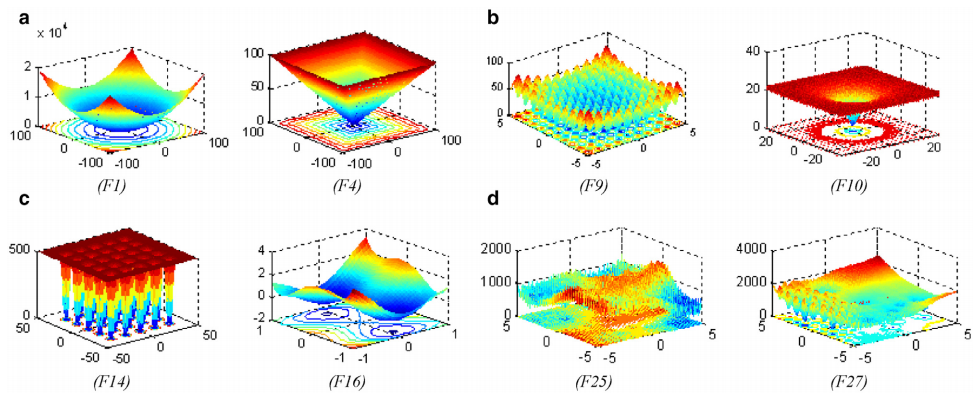
\includegraphics[width=1\textwidth]{pic/whale_function.png}
\end{figure}
\end{frame}

\begin{frame}
  \frametitle{要解决什么优化问题?}
	\begin{itemize}
	\item {实际工程中带有不同约束的优化问题}
	\end{itemize}
\begin{figure}
\centering
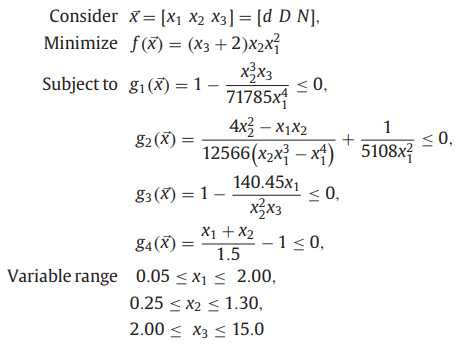
\includegraphics[width=0.6\textwidth]{pic/whale_constraint.png}
\end{figure}
\end{frame}

\begin{frame}
  \frametitle{灵感来源---驼背鲸的捕食行为}
	\begin{block}{制造圆形或螺旋结构的气泡网,收缩包围猎物。}
	\url{http://tv.cntv.cn/video/C36795/3912f2138bca4b15a39c21b17f85116c}
	 \end{block}
\begin{figure}
\centering
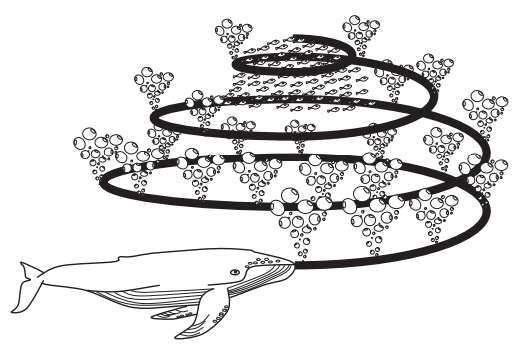
\includegraphics[width=0.6\textwidth]{pic/whale_humpback.png}
\end{figure}

\end{frame}

\begin{frame}
  \frametitle{模型建立}
	\begin{itemize}
	\item {鲸鱼群:在搜索空间中的要搜索的位置}
	\item {猎物:最优解所在位置}
	\end{itemize}
	\begin{block} {\qquad 即在搜索空间中用一群鲸鱼,围绕着当前搜索到的猎物(局部最优解)不断移动位置(迭代更新搜索位置),去寻找猎物更多的位置(最优解)。}
	    \vspace{3mm}
	     \begin{itemize}
	\item {开发阶段(位置更新策略):圆形收缩、螺旋收缩}
	\item {探索阶段(避免局部最优):从比当前位置离局部最优解更远的位置向局部最优解收缩包围}
	\end{itemize}
	\end{block}
	
\end{frame}

\begin{frame}
	\frametitle{模型建立---开发阶段(圆形收缩)}
	\begin{block}{
		\begin{displaymath} \vec{D}= \left | \vec{C}\cdot\vec{X^{*}}(t)-\vec{X}(t) \right | \eqno(1)  \end{displaymath}
		\begin{displaymath} \vec{X}(t+1)=\vec{X^{*}}(t)-\vec{A}\cdot \vec{D} \eqno(2)  \end{displaymath}
	}
	\begin{itemize}
		\item $t$当前迭代    \qquad $\vec{A},\vec{C}$系数向量
		\item $\vec{X^{*}}$当前局部最优解的位置向量,不断更新局部最优解
		\item $\vec{X}$位置向量
		\item $\left | \right |$绝对值    \qquad$\cdot$对应元素相乘
	\end{itemize}
	\end{block}
	\begin{block}{
	\begin{displaymath} \vec{A}=2\vec{a}\cdot\vec{r}-\vec{a} \eqno(3)\end{displaymath}
	\begin{displaymath} \vec{C}=2\cdot\vec{r} \eqno(4)\end{displaymath}
	}
	\begin{itemize}
		\item $\vec{a}$随着迭代过程,从2到0线性递减的向量
		\item $\vec{r}$随机向量,值在[0,1]之间
	\end{itemize}
	\end{block}

	
\end{frame}

\begin{frame}
  \frametitle{模型建立---开发阶段(圆形收缩)图示}
\begin{figure}
\centering
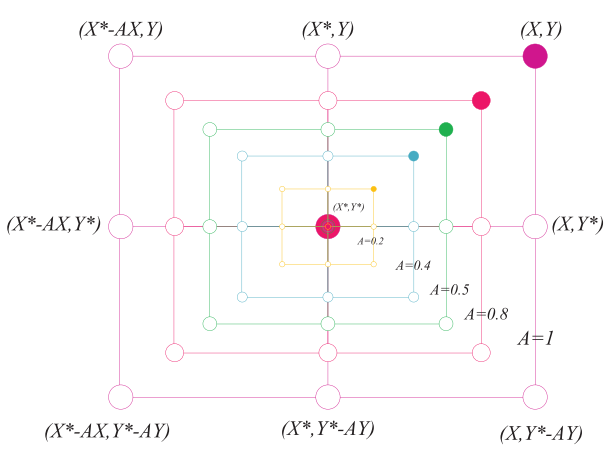
\includegraphics[width=0.6\textwidth]{pic/whale_exploitation1.png}
\end{figure}
\end{frame}

\begin{frame}
  \frametitle{模型建立---开发阶段(螺旋收缩)}
	\begin{block}{
	\begin{displaymath} \vec{X}(t+1)=\vec{{D}'}\cdot e^{bl}\cdot cos(2\pi l)+\vec{X^{*}}(t) \eqno(5)\end{displaymath}}
	\begin{itemize}
		\item $\vec{{D}'}=|\vec{X^{*}}(t)-\vec{X}(t)|$某个鲸鱼离局部最优解的距离(向量的绝对值)
		\item $b$常数,定义对数螺线
		\item $l$随机数,值在[-1,1]
		\item $\cdot$对应元素相乘
	\end{itemize}
	\end{block}
	
\end{frame}

\begin{frame}
  \frametitle{模型建立---开发阶段(螺旋收缩)图示}
\begin{figure}
\centering
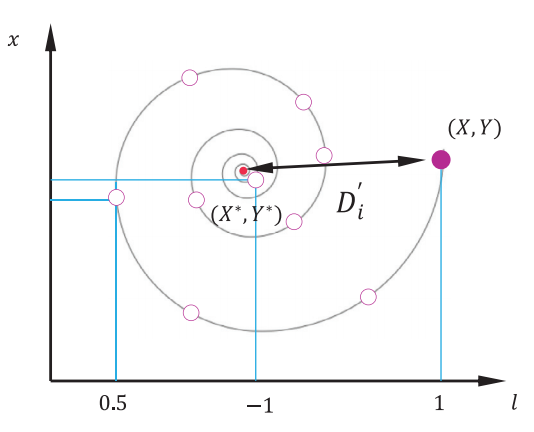
\includegraphics[width=0.6\textwidth]{pic/whale_exploitation2.png}
\end{figure}
\end{frame}

\begin{frame}
  \frametitle{模型建立---开发阶段(两种方式结合)}
	\begin{block}{ 
	\begin{displaymath}
	\vec{X}(t+1)=\begin{cases}
	\vec{X^{*}}(t)-\vec{A}\cdot \vec{D} & \text{ if } p<0.5 \\ 
	\vec{{D}'}\cdot e^{bl}\cdot cos(2\pi l)+\vec{X^{*}}(t) & \text{ if } p\geq 0.5 
	\end{cases}
	\eqno(6)\end{displaymath}
  }
  \begin{itemize}
		\item $p$随机数,值在[0,1]
	\end{itemize}
  \end{block}
 \end{frame}


\begin{frame}
  \frametitle{模型建立---探索阶段(避免局部最优)}
	\begin{block}{
	\begin{displaymath} \vec{D}=|\vec{C}\cdot \vec{X}_{rand}-\vec{X}| \eqno(7)\end{displaymath}
	\begin{displaymath} \vec{X}(t+1)=\vec{X}_{rand}-\vec{A}\cdot \vec{D} \eqno(8)  \end{displaymath}
	}
	\begin{itemize}
		\item $\vec{X}_{rand}$一个随机位置(一条随机的鲸鱼)
	\end{itemize}
	\end{block}
	
\end{frame}

\begin{frame}
  \frametitle{模型建立---探索阶段(避免局部最优)图示}
	\begin{figure}
\centering
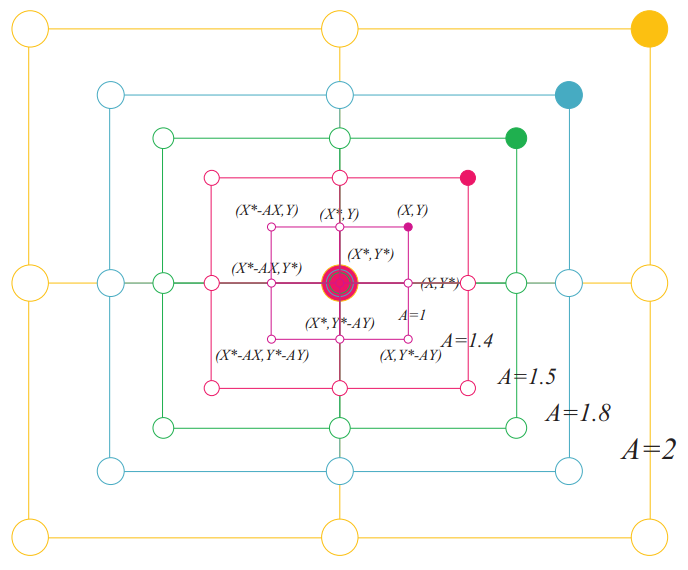
\includegraphics[width=0.6\textwidth]{pic/whale_exploration.png}
\end{figure}
	
\end{frame}



\begin{frame}
  \frametitle{算法步骤}
 Initialize\ the\ whales\ population\ $X_{i}$ (i = 1, 2, ..., n)\\
 Calculate\ the\ fitness\ of\ each\ search\ agent\\
 $X^{*}$=the\ best\ search\ agent\\
 \textbf{\emph{while}} (t < maximum\ number\ of\ iterations)\\
 \qquad \textbf{\emph{for}}\ each\ search\ agent\\
 \qquad Update\ a, A, C, l, and\ p\\
 \qquad \qquad \textbf{\emph{if1}} (p<0.5)\\
 \qquad \qquad \qquad \textbf{\emph{if2}} (|A| < 1)\\
 \qquad \qquad \qquad \qquad Update\ the\ position\ of\ the\ current\ search\ agent\ by\ the\ Eq. (2)\\
 \qquad \qquad \qquad \textbf{\emph{else if2}} ($|A|\geq 1$)\\
 \qquad \qquad \qquad \qquad Select\ a\ random\ search\ agent ($X_{rand}$)\\
 \qquad \qquad \qquad \qquad Update\ the\ position\ of\ the\ current\ search\ agent\ by\ the\ Eq. (8)\\
 \qquad \qquad \qquad \textbf{\emph{end if2}}\\
 \qquad \qquad \textbf{\emph{else if1}} ($p\geq  0.5$)\\
 \qquad \qquad \qquad Update\ the\ position\ of\ the\ current\ search\ by\ the\ Eq. (5)\\
 \qquad \qquad \textbf{\emph{end if1}}\\
 \qquad \textbf{\emph{end for}}\\
\end{frame}

\begin{frame}
  \frametitle{算法步骤}

 \qquad Check\ if\ any\ search\ agent\ goes\ beyond\ the\ search\ space\ and\ amend\ it\\
 \qquad Calculate\ the\ fitness\ of\ each\ search\ agent\\
 \qquad Update\ $X^{*}$\ if\ there\ is\ a\ better\ solution\\
 \qquad $t=t+1$\\
 \textbf{\emph{end while}}\\
 return X*
\end{frame}


\begin{frame}
  \frametitle{评价}
\begin{block}{相较于PSO(粒子群)、GSA(引力搜索)、DE(差分进化)、FEP(快速进化规划)、CMA-ES(协方差矩阵自适应进化)等算法
	}
	\begin{itemize}
		\item 开发能力(单峰函数优化能力)
			\begin{itemize}
				\item 大多测试函数上,排第一到第二位。
			\end{itemize}
		\item 探索能力(多峰函数优化能力)
		\begin{itemize}
				\item 大多测试函数上,排第一到第二位。
			\end{itemize}
		\item 跳出局部最优能力
		\begin{itemize}
				\item 3/7测试函数排第一,3/7个函数问题排第二。
			\end{itemize}
		\item 收敛行为
		\begin{itemize}
				\item 在某些函数上,呈现出较快的后期收敛速度。
			\end{itemize}
	\end{itemize}
	Mirjalili S, Lewis A. The Whale Optimization Algorithm[J]. Advances in Engineering Software, 2016, 95:51-67.
	\end{block}
	
\end{frame}


